\documentclass{article}
\usepackage[UTF8]{ctex}
\usepackage{pythonhighlight}
\usepackage{markdown}
\usepackage{listings}
\lstset{
    basicstyle          =   \tt,          % 基本代码风格
    identifierstyle=\color{brown!80!black},
    keywordstyle        =   \color{purple}\bfseries,          % 关键字风格
    commentstyle        =   \rmfamily\itshape,  % 注释的风格,斜体
    stringstyle         =   \ttfamily,  % 字符串风格
    flexiblecolumns,                % 别问为什么,加上这个
    numbers             =   left,   % 行号的位置在左边
    showspaces          =   false,  % 是否显示空格,显示了有点乱,所以不现实了
    numberstyle         =   \zihao{-5}\ttfamily,    % 行号的样式,小五号,tt等宽字体
    showstringspaces    =   false,
    captionpos          =   t,      % 这段代码的名字所呈现的位置,t指的是top上面
    frame               =   lrtb,   % 显示边框
    backgroundcolor=\color[RGB]{245,245,244},
}


% Language setting
% Replace `english' with e.g. `spanish' to change the document language
\usepackage[english]{babel}
\usepackage{float}
% Set page size and margins
% Replace `letterpaper' with `a4paper' for UK/EU standard size
\usepackage[letterpaper,top=2cm,bottom=2cm,left=3cm,right=3cm,marginparwidth=1.75cm]{geometry}

% Useful packages
\usepackage{amsmath}
\usepackage{graphicx}
\usepackage[colorlinks=true, allcolors=blue]{hyperref}

\title{普物虚拟实验报告2}
\author{雷远航 \ 学号:3210105807}

\begin{document}

\maketitle

\begin{abstract}
    光纤传感器实验
\end{abstract}

\section*{一、实验目的}
\subsubsection*{- 了解光纤的基本知识}
\subsubsection*{- 掌握光纤耦合的计算方法}
\subsubsection*{- 掌握利用光纤的相位调制原理制作相关传感器}



\section*{二、实验原理}

\subsection*{光纤的基本知识:}
纤芯的折射率必须比包层的折射率大,这样才会产生全反射。
$\varphi = arcsin(\frac{n_{2}}{n_{1}})$
    
在光纤断面上,当光线入射角小于一个定值时,折射光线在纤芯和包层界面的入射角$\varphi$才会大于临界角,
光线才能在光纤内多次全反射而传递到另一端。光纤的数值孔径NA
\begin{figure}[H]
    \centering
    
\includegraphics[width=0.9\textwidth]{p3.png}
    \end{figure}

\subsection*{光纤的耦合}
光纤与光源的耦合:直接耦合和经聚光器件耦合。
光耦合效率与光纤端面质量和耦合透镜的数值孔径有关,当光纤断面处理的质量较
好,数值孔径与耦合透镜数值孔径相匹配时可得到最佳耦合效率.这种耦合方法能提
高耦合效率。耦合效率η的计算公式为

\begin{figure}[H]
    \centering
    
\includegraphics[width=0.9\textwidth]{p4.png}
    \end{figure}

\subsection*{光纤干涉仪的相位调制机制}
\begin{figure}[H]
    \centering
    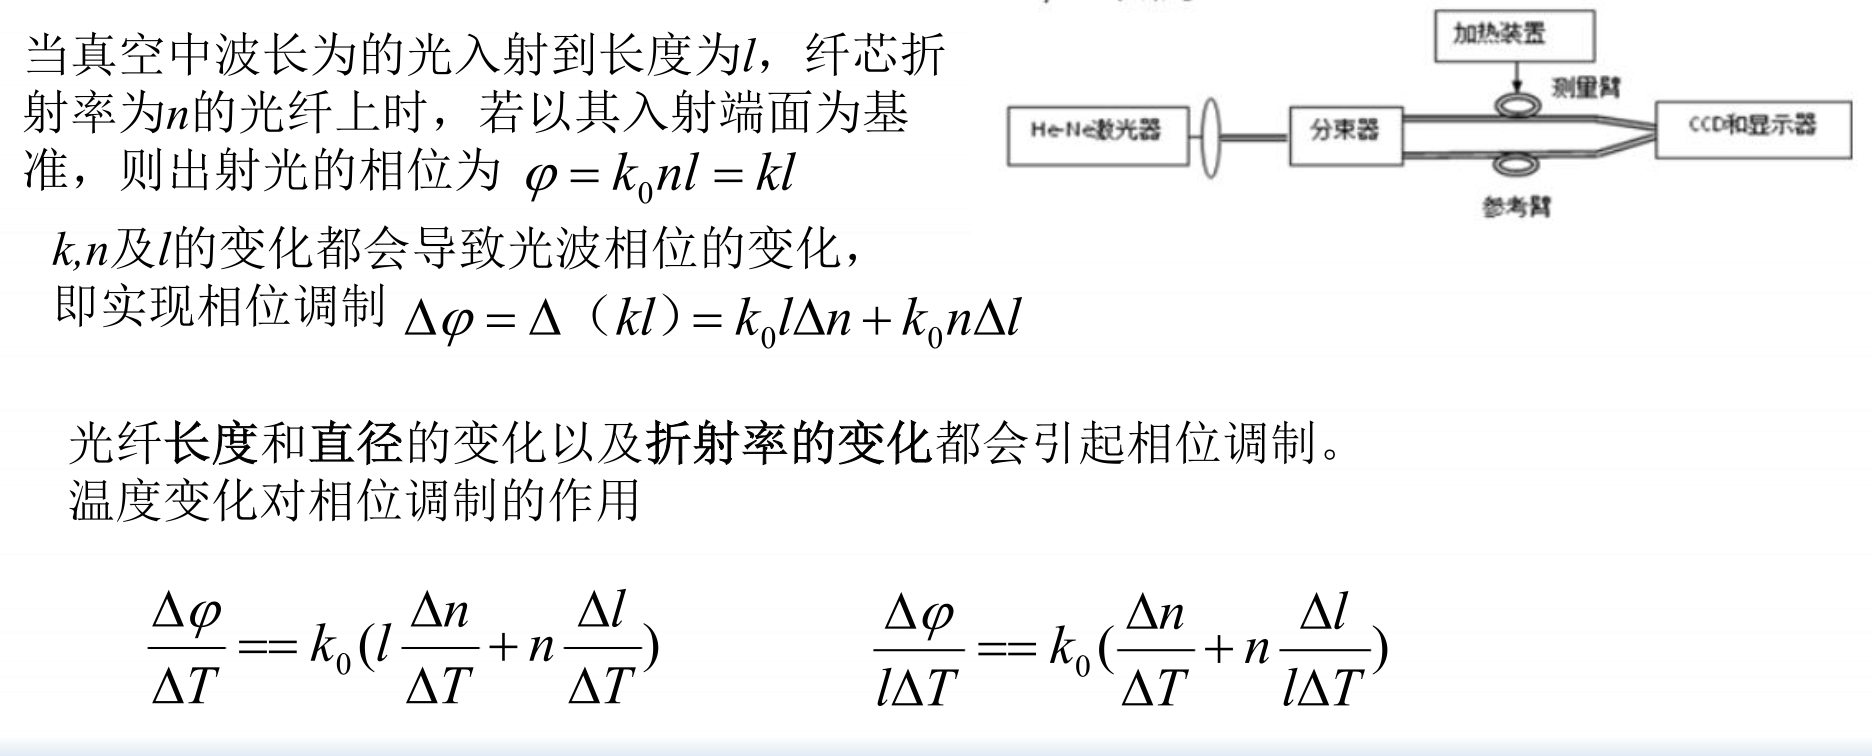
\includegraphics[width=0.9\textwidth]{p5.png}
    \end{figure}

\subsection*{光纤干涉仪的结构与测温原理}
\begin{figure}[H]
    \centering
    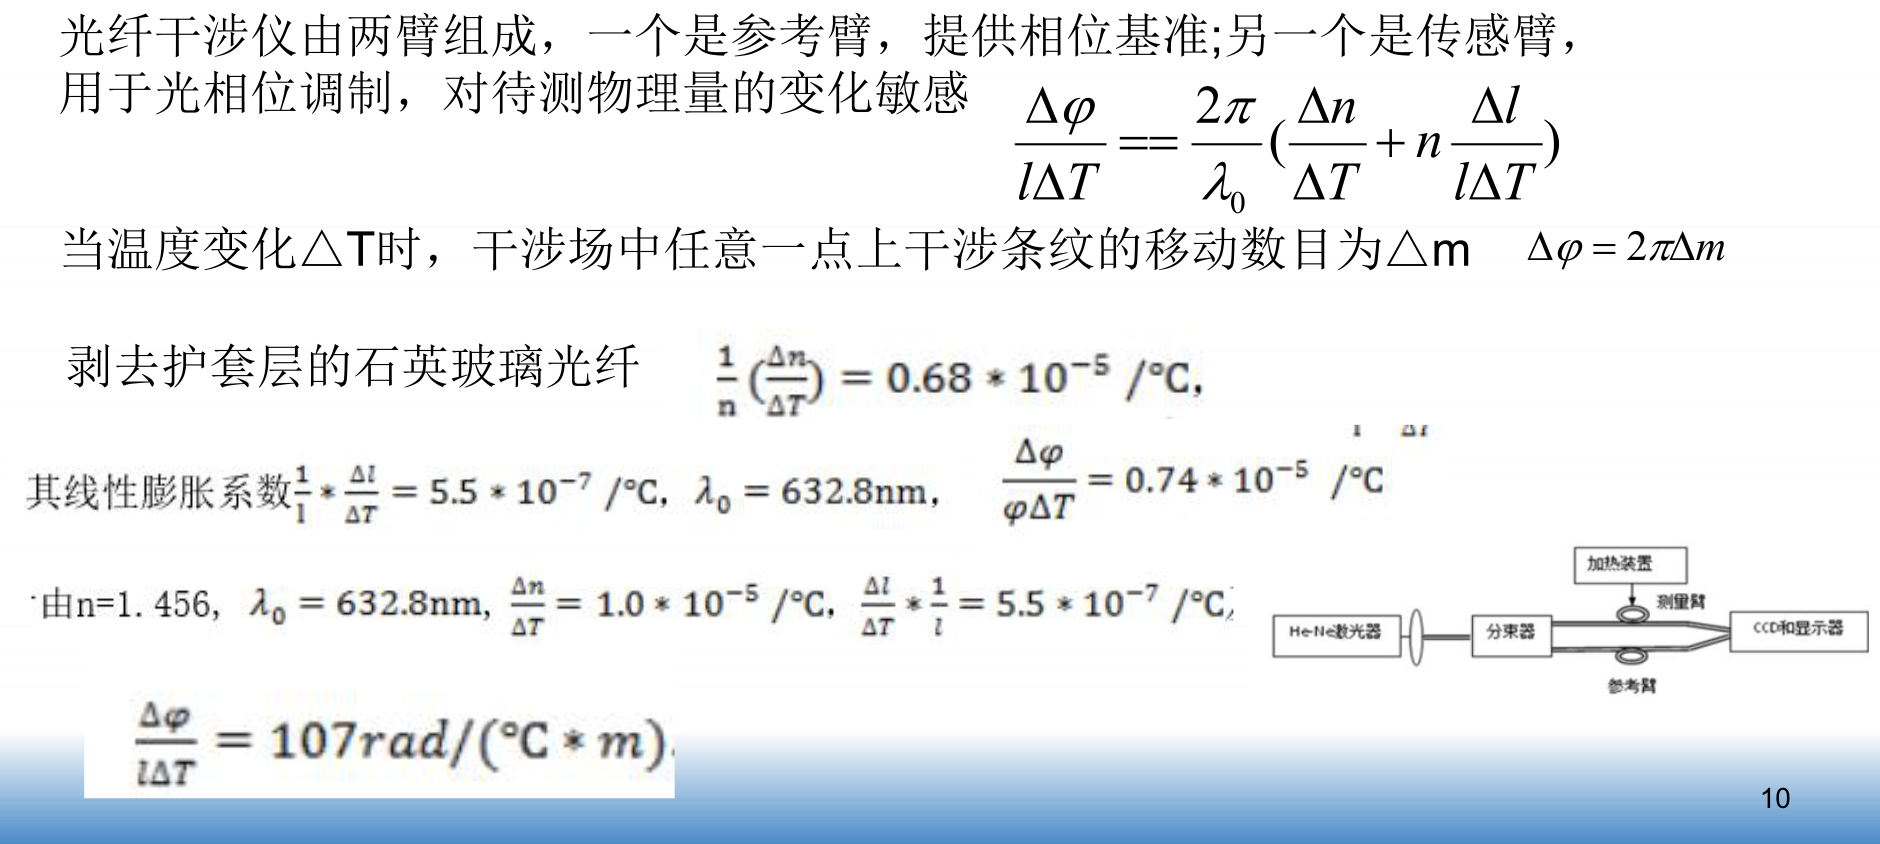
\includegraphics[width=0.9\textwidth]{p6.png}
    \end{figure}

\section*{三、实验数据}

\subsection*{光纤耦合效率计算:}
实验过程中数据记录的截图:
\begin{figure}[H]
    \centering
    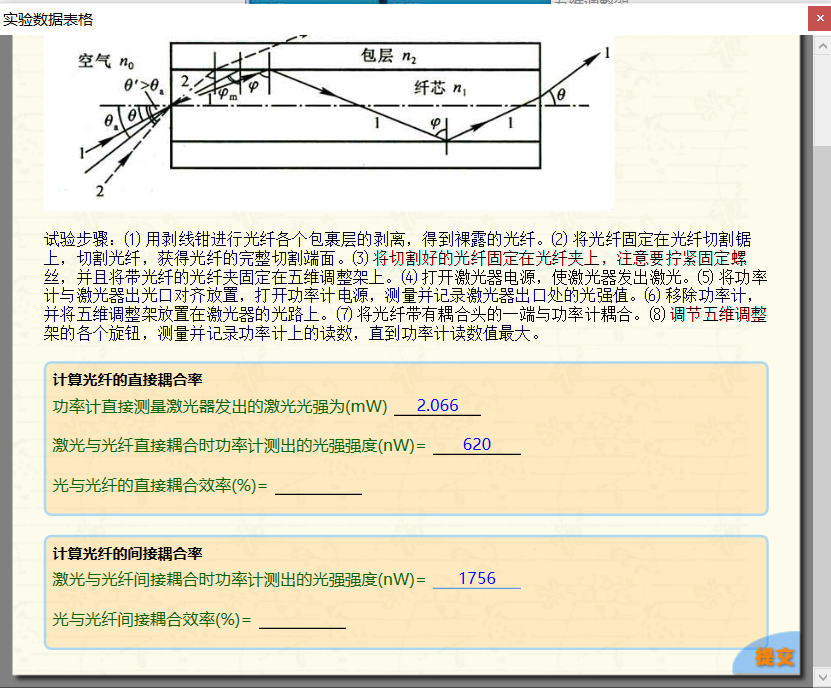
\includegraphics[width=0.9\textwidth]{虚拟2/1.png}
    \end{figure}

由光纤耦合效率的计算公式:$\mu=\frac{P1}{P2}\times$100\%

光与光纤的直接耦合效(\%)=0.0300

光与光纤的间接耦合效(\%)=0.0849 

\subsection*{光纤传感器实验:}

观察清晰的干涉条纹:
\begin{figure}[H]
    \centering
    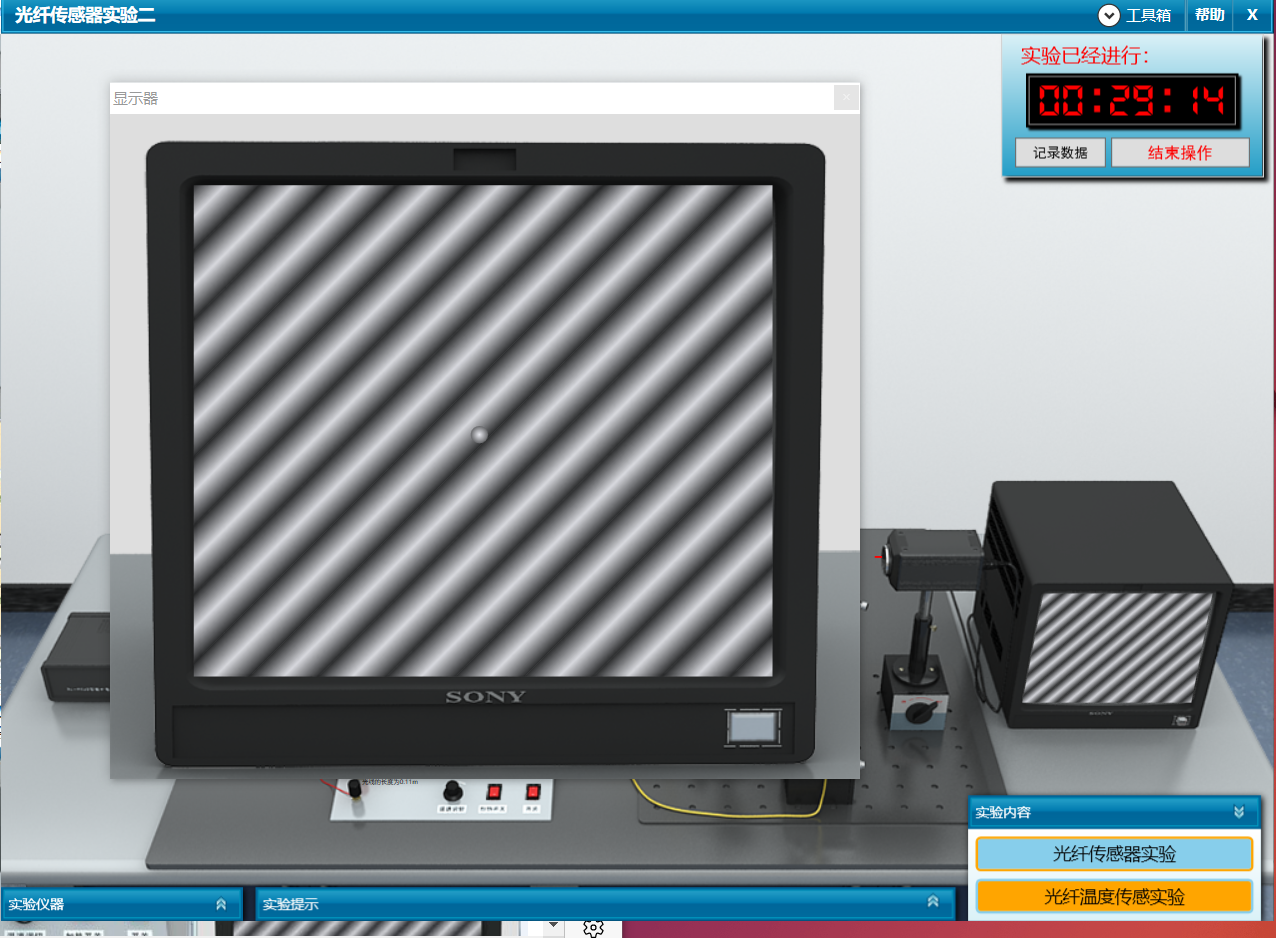
\includegraphics[width=0.9\textwidth]{虚拟2/2.png}
    \end{figure}

实验数据截图:
\begin{figure}[H]
    \centering
    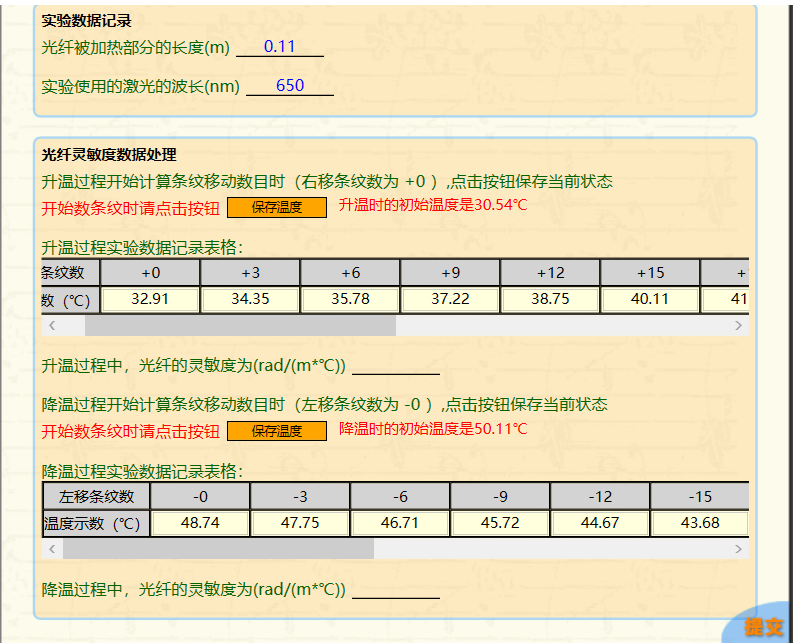
\includegraphics[width=0.9\textwidth]{虚拟2/3.png}
    \end{figure}


\subsubsection*{计算升温光纤温度灵敏度:}

\subsubsection*{作图法:}
利用作图法进行计算:

\begin{figure}[H]
    \centering
    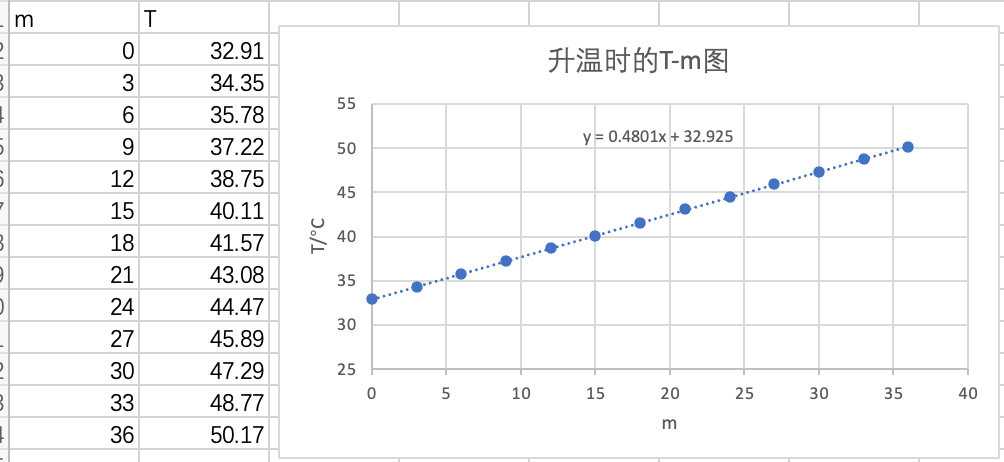
\includegraphics[width=0.9\textwidth]{p1.png}
    \end{figure}
$\frac{\triangle\varphi}{l\triangle{T}}$=$\frac{2\pi\triangle{m}}{l\triangle{T}}$

通过作图可知:$\frac{\triangle{m}}{\triangle{T}}$ = 2.0828

将数据进行带入可知:$\frac{\triangle\varphi}{l\triangle{T}}$ = 118.969(rad/m*°C)


\subsection*{逐差法:}
通过逐差法计算得到:$\frac{\triangle{m}}{\triangle{T}}$ = 2.11

$\frac{\triangle\varphi}{l\triangle{T}}$=$\frac{2\pi\triangle{m}}{l\triangle{T}}$ = 120.522(rad/m*°C)

\subsubsection*{计算降温时光纤温度灵敏度}
\subsubsection*{作图法:}
利用作图法进行计算
\begin{figure}[H]
    \centering
    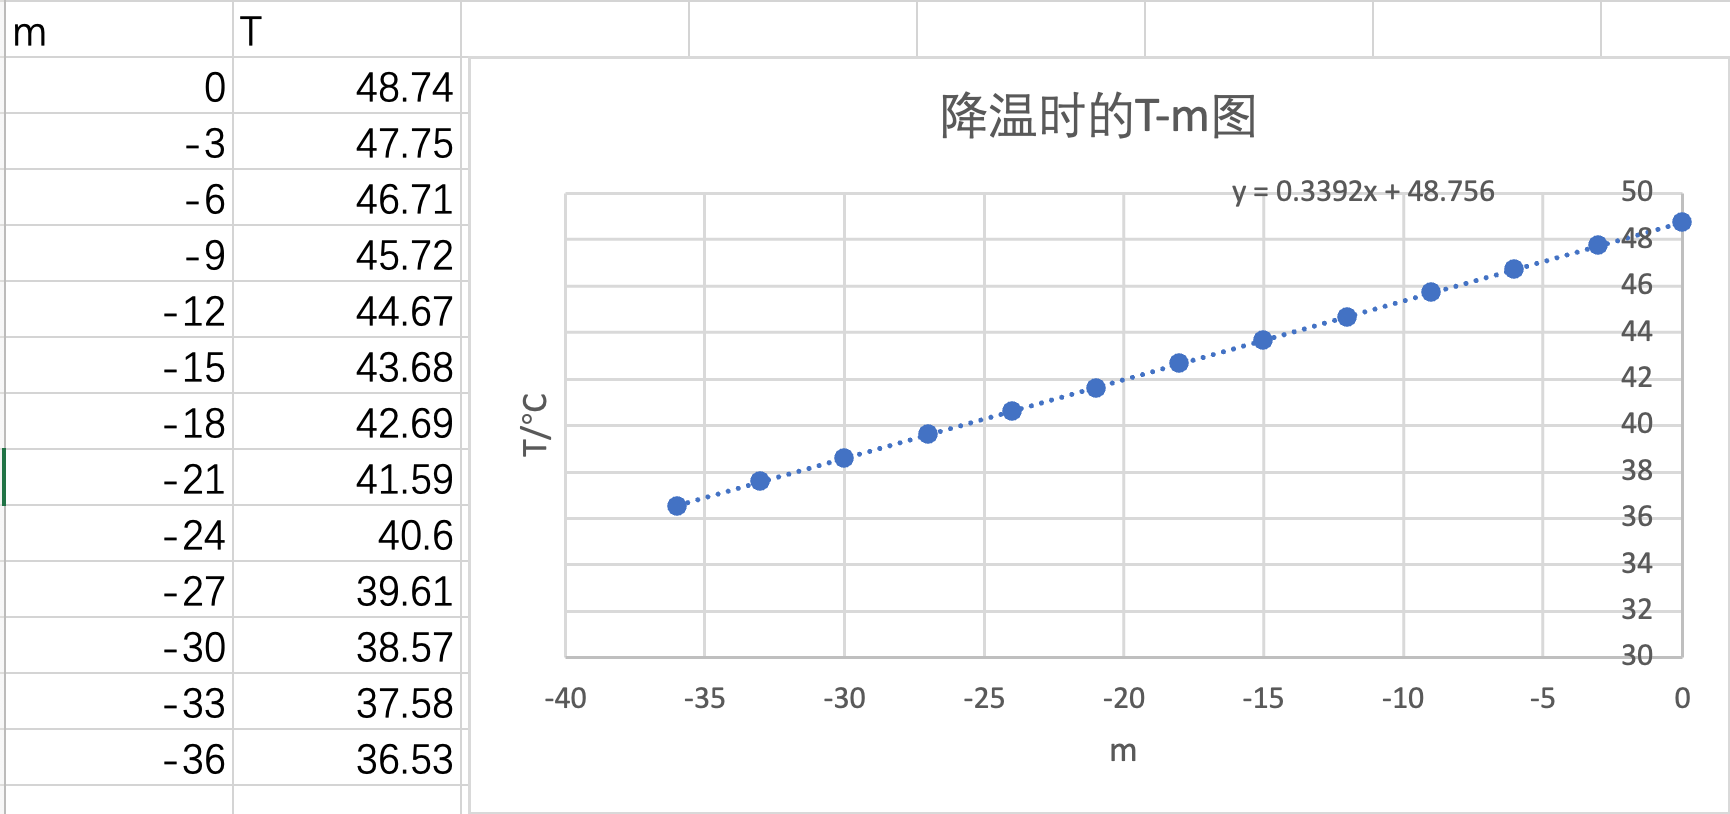
\includegraphics[width=0.9\textwidth]{p2.png}
    \end{figure}

    $\frac{\triangle\varphi}{l\triangle{T}}$=$\frac{2\pi\triangle{m}}{l\triangle{T}}$

    通过作图可知:$\frac{\triangle{m}}{\triangle{T}}$ = 2.94811
    
    将数据进行带入可知:$\frac{\triangle\varphi}{l\triangle{T}}$ = 168.397(rad/m*°C)
    
\subsubsection*{逐差法:}
通过逐差法计算得到:$\frac{\triangle{m}}{\triangle{T}}$ = 2.81

$\frac{\triangle\varphi}{l\triangle{T}}$=$\frac{2\pi\triangle{m}}{l\triangle{T}}$ = 160.507(rad/m*°C)

\section*{四、总结与分析}

\subsection*{思考题}

\subsubsection*{1.能否不用分束器做该实验?是否有替代方案是什么?}
可以,只要用两个相同的相干波波源分别照射光纤即可,这样也可以造成光的干涉.

\subsection*{2.温度改变 1℃ 时,条纹的移动量与哪些因素有关?}
(1)与光纤的温度灵敏度有关
(2)与光纤置于温度场的长度有关

\subsection*{3.温度改变 1℃ 时,条纹的移动量与哪些因素有关?}

可以,可以用透镜将干涉条纹成像在光电探测器上进行测量.

\subsection*{4.标定干涉仪光纤温度灵敏度的误差主要来源是什么?}
光纤被加热部分的长度,实验使用的激光的波长,以及进行读数时的准确性质.

\subsection*{5.在测温光纤传感器的测量臂感温段光纤上粘贴一金属片,其温度灵敏
度会如何变化?}
会影响传感器的响应速度,不会影响传感器的灵敏度。灵敏度(响应量与对应的待测量之比)是传感器的固有特性。光纤温度传感器,直接反映的并不是被测温度,而是自身的温度。只是在测量过程中,传感器被加热(冷却)到和被测温度一致时,传感器自身温度和被测温度相同时,自身温度就代表了被测温度。在温度传感器上贴金属片,会影响传感器被加热(冷却)到和被测温度一致的时间,但不会影响传感器本身的灵敏度。


\subsection*{实验总结}
通过本次线上实验我对光纤的知识有了一定的了解,并且观察了光纤干涉的现象,在计算光纤温度灵敏度时
由于条纹的变化速度有一些快所以在读数的时候有时候总是看错,应当对温度进行即使有效的控制.


\end{document}